\documentclass[../dejiny-rodu-prusiku.tex]{subfiles}

\begin{document}

% str 181 @ 208
\chapter{Větev Červená Řečice}

Zakladatel František Prusík

1789 - 1838

Tato rodová větev je nazvaná po městečku Červené Řečici u Pelhřimova, kde krátce působil a zemřel její zakla­datel František Prusík. Zmínili jsme se již o něm na straně 14 v kapitolce "Plasy a náš rod".
František Prusík byl synem stavitele Martina Prusíka narozeného v roce 1745 v Sedlci. František narodil se v Plasích, kde byl jeho otec usazen, 22. srpna 1789. Bylo to tedy ještě za panovaní císaře Josefa II. U otce se vyučil zednickému řemeslu a později se usadil v Nebřežinech. Tam v roce 1728 zemřel jeho příbuzný hostinský Václav Prusík z Plas, také rodák ze Sedlice. František Prusík byl velmi podnikavým člověkem, ale život neměl dlouhý. Když byl mladý, začalo se v té době u nás objevovati uhlí, jako nové palivo. Lidé nehledali jen na Ostravsku, Mostecku a Kladensku, ale i na Plzeňsku. Vždyť tento nový, zázračný zdroj tepla byl zá­kladnou pro budování velkých průmyslů. A tu se podaři­lo v roce 1819 Františku Prusíkovi objeviti toto černé zlato také v okolí jeho rodiště, v Kaznějově. Nebyl ovšem úplně sám při tomto objevu, ale pomáhali mu zvláště Gűtter a Starck. Z tohoto vzácného objevu uhlí neměl František Prusík žádný materielní zisk. Dnes mu patří za to jen dík, vždyť vše to bylo důvodem k vybudování velkého průmyslu v Kaznějově v pozdějších dobách. Téměř všechno ovoce tohoto objevu sklidil podnikavý žid Starck. Ten se pak stal nejen majitelem průmyslu v Kaznějově, na Radnicku, ale i u Falknova (Sokolov) a jinde.

František Prusík věnoval se dále svému zednickému řemeslu a stal se velmi zručným stavitelem. Důlní právo, které dostal 22. 9. 1819 jako jediný oprávněný majitel objevených ložisek uhlí mu nebylo vlastně nic platné.

František Prusík oženil se v roce 1816 s Josefou Gűtterovou, která se narodila v Nebřežinech 14. 2. 1796. Byla to dcera důchodního panství v Plasích. V Nebřežinech narodily se jim dvě děti. V roce 1821 dcera Klára a za tři roky syn Emanuel. Klára Prusíková zemřela v mládí roku 1832. František Prusík se svou manželkou Josefou odstěhovali se pak do Červené Řečice u Pelhřimova, tedy vlastně dosti daleko od svého rodného kraje, Plasska.

František Prusík byl v Červené Řečici zednickým mistrem zámecké vrchnosti, kterou představovalo pražské arci­biskupství. Z Nebřežin se odstěhovali kolem roku 1825, ale v Červené Řečici příliš dlouho nežili. Josefa Prusíková roz. Gűtterová zemřela tam 29. 6. 1837 a František Prusík za rok po své ženě 28. 8. 1838. Bylo mu jen 49 let.

František Prusík měl jen jedno dítě, které dospělo. Byl to syn Emanuel. Narodil se 21. 4. 1824. Po jeho osudu
% str 182 @ 209
jsme dlouho pátrali. Bylo sice bezpečně zjištěno, že po něm dnes nikde nežije žádná osoba se jménem Prusík, ale mohl míti také dcery. A tu zvláštní náhodou našla se jeho stopa ve starých seznamech pražských obyvatel. Emanuel Prusík vyučil se krejčím a do smrti svých rodičů žil v Červené Řečici. Pak odešel do Prahy, kde již tehdy působil jeho bratranec Josef Prusík, také rodák z Nebřežin. Byl účetním u známé pražské firmy Wimmer.

Emanuel Prusík oženil se s Františkou Pošmurnou. Narodila se v roce 1824 v Olešné u Rakovníka. Měli spolu jedinou dceru. Byla to Anna narozená v pražské porodnici 26. 7. 1855. Emanuel Prusík se svou manželkou Františkou provozoval svou krejčovskou živnost na Malé Straně a později v Loretánské ulici č. 1 na Hradča­nech. Měl četné zákazníky mezi úředníky a duchovními z Malé Strany a Hradčan. Jeho manželka měla současně módní obchod na Starém Městě, v tehdejší Ovocné ulici, dnešní ul. 28.října. Františka Prusíková, roz. Pošmurná zemřela 20. 12. 1892 a její muž Emanuel Prusík za nece­lé tři roky po ní 10. 9. 1895.

Anna Prusíková dcera Emanuela provdala se za diurnistu Zemského úřadu Ludvíka Franka. Jeho otec byl kostelní­kem u sv. Víta a pocházel ze Spáleného Poříčí. Anna Franková nezanechala však žádných potomků, kteří by přežili deset let. Zemřela záhy ve svých 42 letech dne 26. 2. 1897 v Praze na Hradčanech v Loretánské ulici č. l.

František Prusík, rodák z Plas byl tedy zakladatelem jedné naší rodové větve, ale ta již zcela vymřela úmrtím Anny Frankové, roz. Prusíkové v roce 1897. Tato větev nazvaná "Červená Řečice" je dnes jedinou uschlou větví našeho rodu.

% str 182+1 @ 210
\begin{figure}
\centering
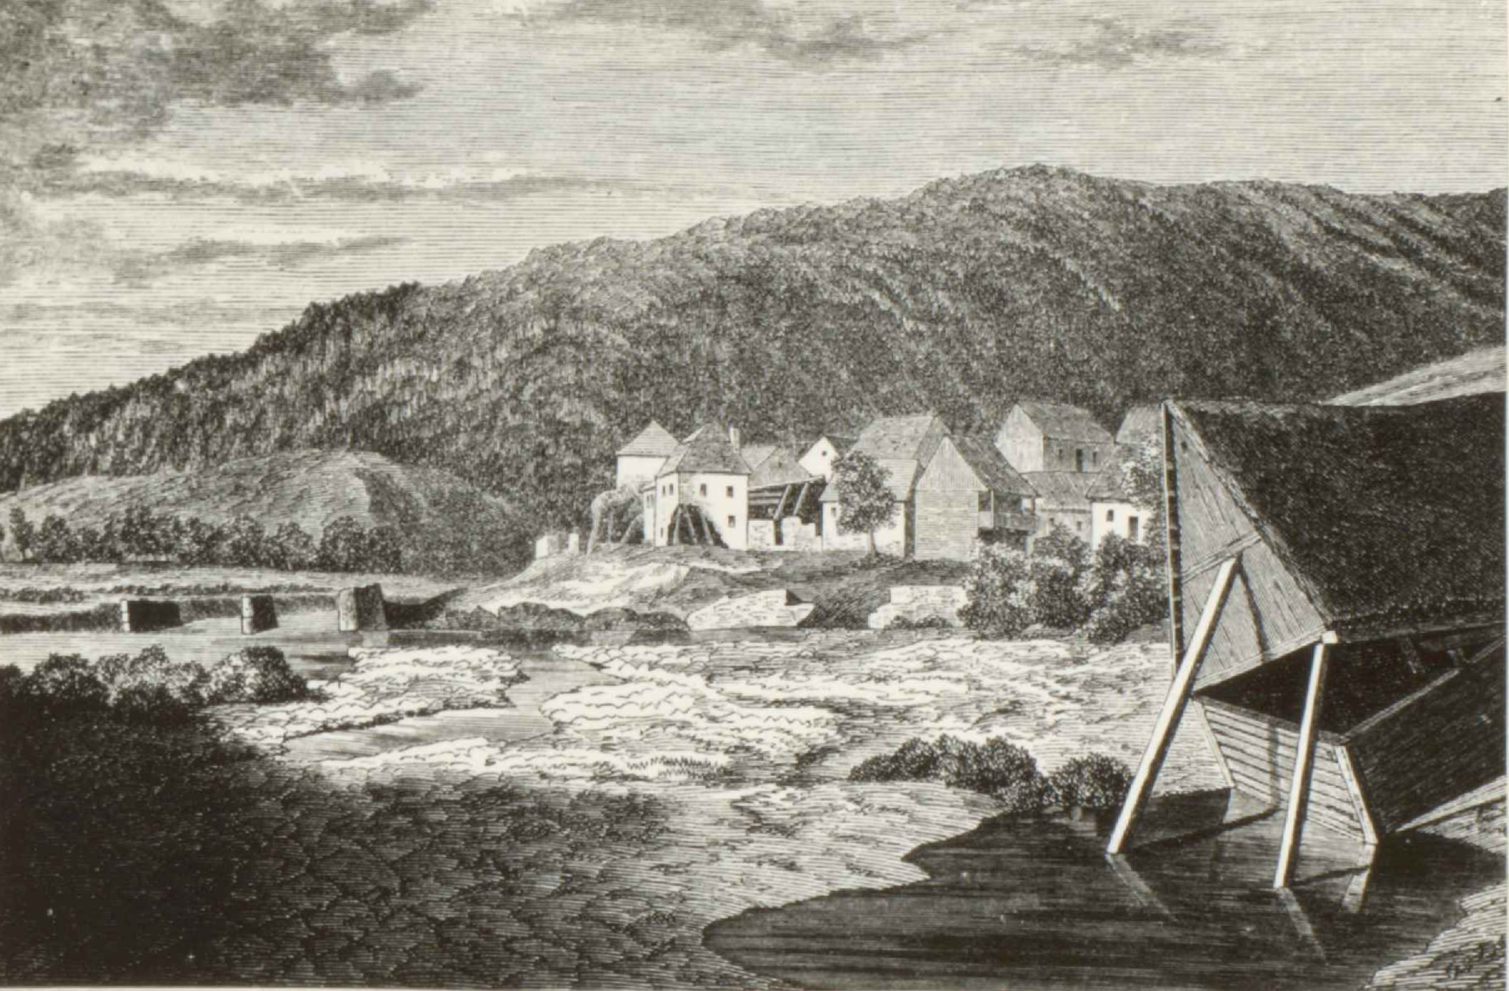
\includegraphics[width=\textwidth, height=\textheight, keepaspectratio]{210-a-nebreziny_po_povodni}
\caption{Tak vypadaly Nebřeziny po povodni roku 1872}
\label{fig:210-a-nebreziny_po_povodni}
\end{figure}

\begin{figure}
\centering
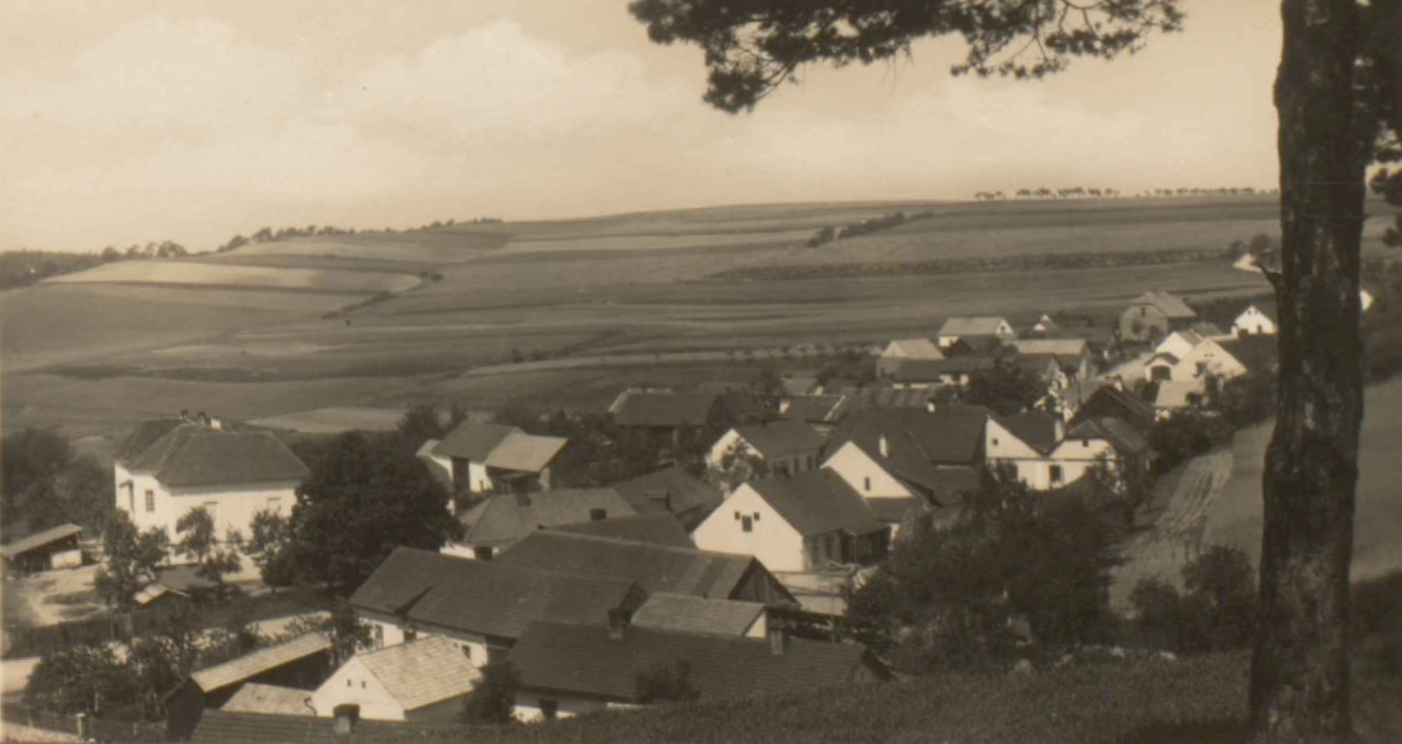
\includegraphics[width=\textwidth, height=\textheight, keepaspectratio]{210-b-nebreziny_sidlo_rodove_vetve}
\caption{Nebřeziny, sídlo rodové větve}
\label{fig:210-b-nebreziny_sidlo_rodove_vetve}
\end{figure}

\end{document}
